\documentclass{report}
\usepackage{hyperref}
\usepackage{graphicx}
\usepackage{enumerate}
\usepackage{enumitem}
\usepackage{xcolor}
\usepackage{import}
\usepackage{pdfpages}
\usepackage{microtype}


\usepackage{geometry}
 \geometry{
 left=1 in,
 right=1 in,
 bottom=1 in,
 top=1 in
}

\setlength\parindent{0pt}

\definecolor{lightGray}{HTML}{d8dde6}

\newcommand*{\backtrack}{\setcounter{enumi}{\numexpr\theenumi-1\relax}}

\title{\textbf{Scholastic Bowl} \\ Round 1 --- Set 2}
\author{Pranaav Sureshkumar \\ \href{mailto:pranaav2@illinois.edu}{pranaav2@illinois.edu}}
\date{\today}

\begin{document}

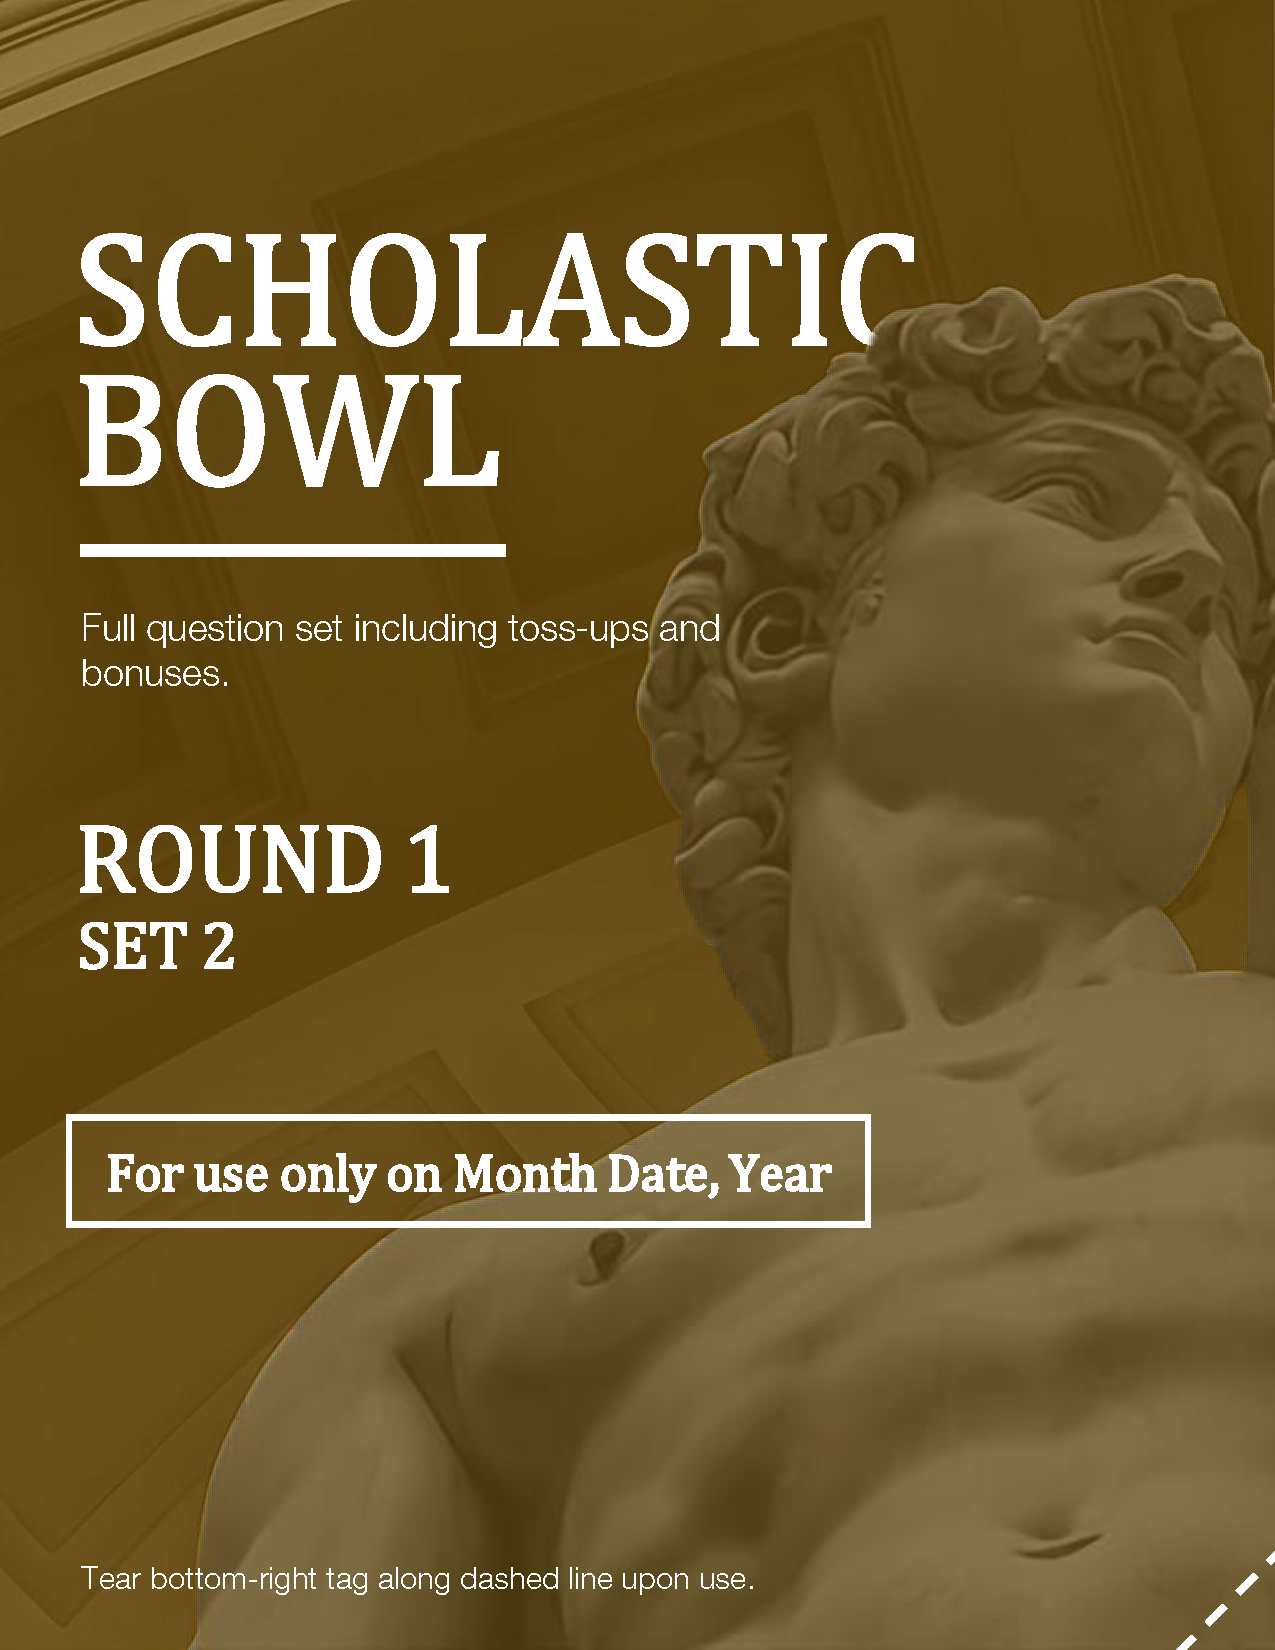
\includepdf[pages=-]{../Title Pages/Round 1 Set 2 Title Page.pdf}

\maketitle

\import{../Rules/}{Rules.tex}

\newpage

\vspace*{\fill}
\centering
\thispagestyle{empty}
\Large
Questions begin on the next page.
\vspace*{\fill}

\normalsize
\newpage
\setcounter{page}{1}

\begin{enumerate}
    % Question 1
    \item \textbf{MATH} \\ \textit{These} processes are called greedy if they always make the locally optimal choice. Turing machines can execute any of \textit{these} processes. Big O notation (*) is used to describe the time and space complexity of \textit{these} processes. For 10 points, name \textit{these} finite, step-by-step sequences of unambiguous instructions that can be used to perform a computation. \\ ANSWER: \underline{algorithm} [prompt on \textit{program}] \backtrack
    \item \textbf{MISCELLANEOUS} \\ Name \textit{these} 1990s bands with prominent drummers. For 10 points each,
    \begin{enumerate}[label=\Alph*]
        \item Dave Grohl drummed on hits like \textit{Heart-Shaped Box} and \textit{Smells Like Teen Spirit} for \textit{this} band. He went on to form the Foo Fighters after the suicide of \textit{this} band’s lead singer, Kurt Cobain. \\ ANSWER: \underline{Nirvana}
        \item Tré Cool replaced John Kiffmeyer in 1990 as \textit{this} band's drummer. He drummed in hits like \textit{Brain Stew}, \textit{American Idiot}, and \textit{Know Your Enemy}. \\ ANSWER: \underline{Green Day}
        \item Chad Smith drummed for \textit{this} band since 1988, producing hits such as \textit{Snow}, \textit{Under the Bridge}, and \textit{Californication}. \\ ANSWER: \underline{Red Hot Chili Peppers}
    \end{enumerate}

    % Question 2
    \item \textbf{SOCIAL SCIENCE} \\ Plato once referred to \textit{these} animals as ``the only featherless bipeds with broad, flat nails (*).'' A philosophical stance named after \textit{these} animals was pioneered by Petrarch. Friedrich Nietzsche \colorbox{lightGray}{[\textbf{Neet}\textperiodcentered shuh]} claimed that \textit{these} animals killed God. For 10 points, name \textit{these} animals which were often the subject of Italian Renaissance art like the \textit{Mona Lisa}. \\ ANSWER: \underline{human}s \backtrack
    \item \textbf{SCIENCE} \\ In mechanical physics, almost all translation quantities have rotational analogues. Name the following quantities and operations used in rotational mechanics. For 10 points each,
    \begin{enumerate}[label=\Alph*]
        \item \textit{This} quantity is the rotational analogue of force. When a force is applied perpendicular to a lever arm, \textit{this} quantity is the force applied multiplied by the distance to the pivot. \\ ANSWER: \underline{torque}
        \item Torque is the rotational analogue of force. Therefore, by Newton's Second Law, it is also equal to angular acceleration multiplied by \textit{this} quantity. \\ ANSWER: \underline{rotational inertia} [also accept \underline{moment of inertia}, \underline{angular mass}, \underline{rotational mass}, or \underline{second moment of mass}]
        \item When the force and lever arm vectors are not perpendicular, \textit{this} vector operation must be used to find torque. Unlike the dot product, this operation yields a vector. \\ ANSWER: \underline{cross} product
    \end{enumerate} 

    % Question 3
    \item \textbf{HISTORY} \\ During the War of 1812, \textit{this} poet watched from a British ship as the American troops in Fort McHenry raised their flag (*). Abolitionists criticized \textit{this} poet's words that America was the land of the free\textemdash instead referring to it as ``the land of the free and the home of the oppressed.'' On March 26, 2024, a Baltimore bridge named after \textit{this} poet collapsed. For 10 points, name \textit{this} poet who wrote \textit{The Star-Spangled Banner}, which later became the US national anthem. \\ ANSWER: Francis Scott \underline{Key} \backtrack
    \item \textbf{MISCELLANEOUS} \\ In French culinary theory, there are \textit{mother} sauces from which many other \textit{daughter} sauces are derived. Name the following mother sauces by the daughter sauces they're used to make. For 10 points each,
    \begin{enumerate}[label=\Alph*]
        \item \textit{This} mother sauce is the base for salsas and many pasta dishes. \\ ANSWER: \underline{tomato} sauce
        \item \textit{This} mother sauce is the base for tartar sauce and ranch dressing. \\ ANSWER: \underline{mayo}nnaise
        \item \textit{This} mother sauce is the base for foyot \colorbox{lightGray}{[foe\textperiodcentered \textbf{yote}]} sauce and is often served with Eggs Benedict. \\ ANSWER: \underline{hollandaise} sauce
    \end{enumerate}

    % Question 4
    \item \textbf{LITERATURE} \\ In \textit{this} cautionary novel, Oceania, Eurasia, and Eastasia are constantly at war, which Emmanuel Goldstein believes is the only way to maintain peace. In \textit{this} novel, Winston Smith is betrayed and captured by secret members of the Thought Police (*) who turn him in to the Party. Four government agencies in \textit{this} novel are ironically named the Ministries of Truth, Peace, Love, and Plenty. For 10 points, name \textit{this} dystopian novel about totalitarianism, written by George Orwell, which popularized terms such as \textit{thoughtcrime}, \textit{doublethink}, and \textit{Big Brother}. \\ ANSWER: \underline{Nineteen Eighty-Four} \backtrack
    \item \textbf{SCIENCE} \\ Every quantity you can think of can be expressed in terms of SI units. Name the following quantities by their definition in SI units. For example, if I said \textit{meters per second}, you would answer \textit{speed} or \textit{velocity}\textemdash both are acceptable. For 10 points each,
    \begin{enumerate}[label=\Alph*]
        \item \textit{This} quantity is measured in meters cubed. \\ ANSWER: \underline{volume} [do \textbf{not} accept or prompt on \textit{liter}]
        \item \textit{This} quantity is measured in ampere-seconds. \\ ANSWER: electric \underline{charge} [do \textbf{not} accept or prompt on \textit{coulomb}]
        \item \textit{This} quantity is measured in kilogram-meters squared per second squared. \\ ANSWER: \underline{energy} [also accept \underline{work} or \underline{torque} or \underline{heat} (but \textbf{not} \textit{temperature}); do \textbf{not} accept or prompt on \textit{joule}]
    \end{enumerate} 

    % Question 5
    \item \textbf{SOCIAL SCIENCE} \\ \textit{This} company, formerly known as \textit{Real-Time Cures} was exposed by John Ioannidis for its exaggerated claims. In response to growing skepticism, executives at \textit{this} company invited Vice President Joe Biden to tour its facilities. Although Joe Biden initially praised the lab, it was later found that the facility was fake and used only to lure investors. Elizabeth Holmes, the CEO of \textit{this} company, claimed its technology could perform thirty distinct tests on a single drop of blood (*). For 10 points, name \textit{this} fraudulent company whose name is derived from a combination of the words \textit{therapy} and \textit{diagnosis}. \\ ANSWER: \underline{Theranos} \backtrack
    \item \textbf{HISTORY} \\ Ulrich Zwingli and John Calvin, among others, rebelled against Catholicism in the Protestant Reformation that began in the 1500s. For 10 points each,
    \begin{enumerate}[label=\Alph*]
        \item Among those who rebelled was \textit{this} German priest who was tried in the Diet of Worms for nailing his \textit{Ninety-five Theses} to the door of a Catholic Church. In doing so, he founded a namesake religion. \\ ANSWER: \underline{Martin Luther} [also accept \underline{Lutheranism}]
        \item In his \textit{Ninety-five Theses}, Martin Luther argues against the effectiveness of \textit{these} items sold by the Catholic Church. Johann Tetzel claimed that these items could be bought to relieve a Catholic from common sins. \\ ANSWER: \underline{indulgence}s
        \item Although theologians like Jan Hus \colorbox{lightGray}{[Yaan Hoose]} had similar ideas, Martin Luther's movement found great success because his message was spread throughout Europe by \textit{this} newly-invented device. \\ ANSWER: \underline{printing press}
    \end{enumerate}

    % Question 6
    \item \textbf{SCIENCE} \\ \textit{This} interaction is, by far, the weakest of the four fundamental interactions. Like the electrostatic force, \textit{this} interaction has infinite range. In his general theory of relativity, Einstein showed that \textit{this} interaction was not a force, but rather the result of the curvature of spacetime. On Earth's surface, \textit{this} interaction's constant of acceleration is 9.8 meters per second squared. For 10 points, name \textit{this} interation which gives weight to all objects on Earth. \\ ANSWER: \underline{gravity} \backtrack
    \item \textbf{FINE ARTS} \\ Name the following structures in Greco-Roman architecture. For 10 points each,
    \begin{enumerate}[label=\Alph*]
        \item \textit{These} structures can be built in the Doric, Ionic, or Corinthian style. They have a base, shaft, and capital and are often used to bear a vertical load. \\ ANSWER: \underline{column} [prompt on \textit{pillar}]
        \item \textit{These} open-air buildings, which are used for entertainment, often feature many columns and arches. Isidore of Seville said that \textit{these} buildings are called what they are because, unlike a traditional theater, \textit{these} structures are round. \\ ANSWER: \underline{amphitheater}
        \item \textit{This} structure is the largest amphitheater that has ever been built. \\ ANSWER: \underline{Colosseum}
    \end{enumerate}

    % Question 7
    \item \textbf{LITERATURE} \\ \textit{This} character owns a sword named Anaklusmos \colorbox{lightGray}{[\textbf{Ann}\textperiodcentered uck\textperiodcentered luss\textperiodcentered moce]}, which transforms from a pen when uncapped. \textit{This} character, whose mother always makes him blue-colored food, is taken by his best friend Grover Underwood to Camp Half-Blood. \textit{This} character journeys to the Underworld with Grover and Annabeth. For 10 points, name \textit{this} son of Poseidon whom Rick Riordan wrote about in \textit{The Lightning Thief}. \\ ANSWER: \underline{Percy Jackson} [prompt on \textit{Percy} or \textit{Jackson} alone] \backtrack
    \item \textbf{MISCELLANEOUS} \\ Name these saws you might find at a woodshop. For 10 points each,
    \begin{enumerate}[label=\Alph*]
        \item \textit{This} saw can be used for crosscutting or ripping, but it is typically used for making curved cuts. Unlike a jigsaw, \textit{this} saw is floor-mounted and features a flexible, looped, blade. \\ ANSWER: \underline{bandsaw}
        \item \textit{This} saw can only make straight cuts. \textit{This} saw is usually the most dangerous saw in a woodshop, but modern safety features like the SawStop can help make it safer. \\ ANSWER: \underline{tablesaw}
        \item \textit{This} saw can only make crosscuts but can do so at an angle. The sliding, compound version of \textit{this} saw can also make bevel cuts. \\ ANSWER: \underline{Miter} saw
    \end{enumerate}


\end{enumerate}


\vspace*{0.5 cm}
\centering
\rule{10 cm}{0.4pt}

\Large
END OF QUESTION SET
\newpage

\vspace*{\fill}
\centering
\thispagestyle{empty}
\Large
No questions on this page
\vspace*{\fill}

\newpage

\vspace*{\fill}
\centering
\thispagestyle{empty}
\Large
No questions on this page
\vspace*{\fill}

\end{document}